% -*-coding: utf-8 -*-

U každé heuristiky popíšeme strom komponent a posléze jejich implementaci. Heuristiky opět popisujeme bez stop podmínky. V diagramech za dvojtečkou uvádíme rodiče dané komponenty, kurzívou popisujeme odpovídající komponentu v dekompozičním formalismu. Kontejner na kandidáty a archiv z diagramů vynecháváme, protože jejich role je jasná. Za účelovou funkci zde volíme sférickou $f(x) = \sum_{i=1}^n x_i^2$ s minimem v $0$.

\section{Náhodná střelba}

Random Shooting je spolu s Hill Climbing nejzákladnější, a také implementačně nejjednodušší heuristikou. Nevyužívá potomstvo, nastavíme tedy jeho velikost na $0$ a všechny operace budeme provádět pouze na populaci. Strom komponent vypadá následovně:

\begin{figure}[h!]
\begin{center}
  \includegraphics[width=\textwidth]{img/RS}
  \caption{Dekomponovaná náhodná střelba}\label{RS dekomp}
  \end{center}
\end{figure}

V kořenu vidíme hlavní objekt algoritmu, dále pak dva wrappery, které říkají, že veškeré operace se budou dít nad populací. Taktéž bychom mohli všechny slave komponenty přidat až pod druhý wrapper, funkčně by se nic nezměnilo. Wrappery v tomto případě nepřinášejí do logiky algoritmu nic nového, a tak ani nemají ekvivalent ve formalismu. Chybějící inicializace je vysvětlena v sekci \ref{def inicializace}.

\subsection{Implementace slave komponent}

Náhodná inicializace je implementována přímočaře. Na CPU je použita funkce \texttt{rand} vracející hodnoty z intervalu [0,RAND\_MAX]\footnote{RAND\_MAX je nejméně 32768, na testovacím serveru bylo RAND\_MAX shodné s INT\_MAX, což je hodnota pro všechny potřeby dostačující.}, což jednoduše transformujeme v každé dimenzi na interval [nižší mez, vyšší mez]. Na stejný interval transformujeme výsledek \texttt{curand\_uniform} na GPU. Implementace ohodnocení sférickou funkcí je stejně přímočará.

Implementačně nejzajímavější z hlediska GPU je archivační komponenta. Archivujeme pouze nejlepšího kandidáta z každé populace v každé generaci spolu s jeho fitness. To vyžaduje počítání minima (fitness), na které můžeme na GPU použít paralelní redukci. Ta při dostatku prostředků spočítá minimum z $n$ prvků v čase $O(\log_2 n)$ oproti $O(n)$ času, který potřebuje sekvenční verze.

\section{Genetická optimalizace}

Dekompozice GO je také jednoduchá, avšak mnohem obsáhlejší, protože obsahuje mnohem více komponent. Strom komponent je na diagramu \ref{GO dekomp}.

\begin{figure}[h!]
\begin{center}
  \includegraphics[width=\textwidth]{img/GO}
  \caption{Dekomponovaná genetická optimalizace}\label{GO dekomp}
  \end{center}
\end{figure}

Nejprve několik komentářů ke vztahu k formalismu. Jednak se zde naplňuje tvrzení, že výsledek je vždy kompromisem mezi formalismem a implementací, a zároveň se zde projevuje volnost, nebo spíše pružnost obou částí. K vztahu model-formalismus: za inicializaci musíme považovat celý wrapper, protože selekce vyžaduje množinu jedinců a tedy samostatná náhodná inicializace ani ohodnocení nemá smysl.

Za mutaci má smysl taktéž označit celý wrapper, protože v případě že mutujeme pouze s jistou pravděpodobností (předána wrapperu v konstruktoru), má na starosti nastavení rozsahu pro obě podkomponenty. Pokud křížíme taktéž jen s jistou pravděpodobností, wrapperu předáme tuto pravděpodobnost a on nastaví rozsahy tak, aby emuloval stochastickou nezávislost obou operací. Pertubaci zavěsíme pod stejný wrapper, protože pouze gaussovská mutace může vybočit z mezí.

Nyní vysvětlíme přerušované čáry u podkomponent sjednocení, oddělení třídění a přesunu bude vysvětleno v implementační části. Sjednocení nahrazením je na rozdíl od jiných komponent svými podkomponentami definováno. Mutace by stále byla mutací, pokud by přičítaný šum měl jiný charakter nebo byla pertubace zrcadlová. Stejně tak reprodukce. Jde zde o nastavování mezí: u mutace stačí říci, že všechny podkomponenty budou pracovat nad jedním rozsahem, u reprodukce bude selekce vždy vybírat z populace a křížení vždy ukládat do potomstva. Sjednocení se od sebe však mohou podstatně lišit: u nahrazení musíme provést setřídění potomstva a nahrazení populace jeho nejlepší částí. V~případě sjednocení s elitismem musíme nejprve setřídit populaci, elitu přesunout na její začátek, poté setřídit potomstvo a jeho nejlepší částí nahradit zbytek populace. Jsou to tedy čtyři operace vyžadující naprosto odlišné nastavení rozsahů. Z těchto důvodů jsou podkomponenty sjednocení přidány již v konstruktoru a nelze s nimi hýbat. Jeden ze~způsobů, jak toto řešit, by bylo rozbourání sjednocení jako takového a nahradit ho jen posloupností třídění (spojených s přesunem) a přesunů. Tím by ovšem klesla efektivita (viz dále).

\subsection{Implementace slave komponent}

Implementace inicializace, ohodnocení a archivace byla popsána v předchozím příkladě.

\subsubsection{Reprodukce -- selekce a křížení}

Jak bylo řečeno, reprodukce pouze nastavuje rozsahy: pro selekci na populaci, pro křížení na potomstvo. Jako uživatelský parametr jí předáváme pravděpodobnost křížení, která určuje, kolik počátečních bodů z potomstva vznikne křížením (zbytek bude jen zkopírován z populace).

Jako selekci jsme zvolili 2-tournament -- z populace jsou vybráni náhodně dva jedinci a~lepší je zařazen do mating pool. Na CPU se toto provádí, dokud není mating pool naplněn, na GPU spustíme kernel s tolika vlákny, kolik je velikost mating pool. Pokud je velikost mating pool příliš velká, spustíme kernel s maximálním počtem vláken (512 nebo 1024) -- pro tento případ je v kernelu cyklus, díky němuž může jedno vlákno naplnit tolik položek mating pool, kolik je třeba. Takto je řešen nedostatek vláken i u ostatních komponent.

Jednobodové křížení probíhá ve dvou fázích: nejprve křížením vytvoříme tolik potomků, kolik odpovídá pravděpodobnosti křížení, zbytek zkopírujeme podle indexů z mating pool. Reprodukce zařídí, aby mating pool obsahoval přesně (2$\times$počet jedinců vzniklých křížením + počet jedinců vzniklých kopírováním) indexů. Bod křížení je pro každého jedince vygenerován náhodně tak, aby vzniklý jedinec obsahoval vždy prvky z obou rodičů. Implementace na GPU je stejná jako popsaná, problémem je jen přístup do paměti. Protože k jedincům přistupujeme přes indexy z mating pool, jde o přístup relativně náhodný, a~tedy i pomalejší. Při zachování náhodnosti to ale jinak řešit nejde.

\subsubsection{Mutace a pertubace}

Opět jde o implementačně jednoduché operace. Gaussovský šum je CPU i GPU generován pomocí Box-Mullerovy transformace, na CPU explicitně vypočtené, na GPU je součástí funkce \texttt{curand\_normal2}. Rozptyl šumu je předán gaussovské mutaci jako uživatelský parametr. Důležitým aspektem pro celočíselné, a speciálně pak pro binární úlohy, je způsob zaokrouhlování. Proto se kritickým komponentám šablonovým parametrem předá třída, která implementuje požadovaný způsob zaokrouhlování. V našem případě bylo použito zaokrouhlení pravděpodobnostní, tedy $x$ je zaokrouhleno nahoru s pravděpodobností $p = x - \text{floor}(x)$, jinak je zaokrouhleno dolů.

Pertubaci jsem volili periodickou, implementace je zřejmá.

\subsubsection{Sjednocení -- třídění a přesun}

První částí sjednocení nahrazením je třídění. Je nutné si uvědomit, že výstupem třídění není množina jedinců setříděná podle fitness, ale pouze \emph{množina indexů jedinců setříděná podle fitness}. Má to několik důvodů: jedinec může být relativně velký objekt a je zbytečné ho několikrát přesouvat, když to stačí udělat jednou. Na GPU se tento nevýhodný efekt ještě znásobí, uvážíme-li, že přesuny jsou značně náhodné. Navíc v případě sjednocení nahrazením bychom zbytečně třídili množinu, ze které budeme jen část kopírovat a poté jí zahodíme.

Pro implementaci na GPU jsme použili osvědčené Bitonické třídění (BT), jehož popis lze najít například na wikipedii \cite{Bitonic}. Paralelní složitost BT je $O(\log_2^2 n)$. Na CPU pak \texttt{partial\_sort} ze standardní knihovny STL. Implementaci BT jsme pojali nejjednodušším možným způsobem. Z toho plyne omezení velikosti tříděné množiny na $2^k$, což pro pro běžně používané velikosti potomstva u GO není problém -- velikost stačí případně zaokrouhlit na nejbližší (vyšší) mocninu dvou. Pokud by byl počet jedinců, a s tím související počet vyčíslení fitness, kritický, bylo by dobré implementovat BT pro libovolnou velikost množiny. Na GPU vždy třídíme celou množinu, což je algoritmicky jednodušší, zatímco na CPU setřídíme jen část, kterou pak bude nahrazena populace.\vspace{0.2cm}

Přesun je v našem případě bez problémů, protože cílová a zdrojová množina jsou disjunktní. V jiné komponentě by tomu ale tak být nemuselo a při sekvenčním přístupu by se nám mohlo stát, že přepíšeme data, která ještě budeme potřebovat. V paralelním kódu by mohla nastat podobně nebezpečná read-before-write situace\footnote{Správnost výsledku závisí na to, jestli se dřív vykoná čtení jedním vláknem, nebo zápis druhým. Pořadí operací různých vláken však není definované.}. Aby byl in-place přesun bezpečný i pokud jsou zdrojová cílová množina stejné, je nutné v sekvenčním kódu konflikty eliminovat, což při zachování částečného setřídění lze. Na GPU nejprve data zkopírujeme do sdílené paměti a poté na místo určení, protože řešení konfliktů by v~paralelním kódu nebylo efektivní.

\section{Diferenciální evoluce}

Diferenciální evoluce má stejný strom komponent jako GO, liší se jen slave komponentami selekce, křížení a komponentou sjednocení. Sjednocení je vyžadováno jako souboj potomka s přímým rodičem (velikost populace a potomstva je stejná). Bude tedy obsahovat wrapper, který nastaví \texttt{workingRange} na populaci a \texttt{fullRange} a samotnou slave komponentu sjednocení.

\subsection{Implementace slave komponent}

\subsubsection{Selekce}

Do mating pool budeme vybírat pouze indexy jedinců $a,b,c$ z definice DE. Velikost mating pool bude tedy trojnásobek velikosti potomstva, a tedy i populace. Nejprve naplníme za~pomoci co nejvíce vláken náhodně celý mating pool. Potom za pomoci $n = |Q|$ vláken postupně ověříme podmínky:
\begin{itemize}
  \item Pokud $x == a$ ($x$ bude odpovídat ID threadu), inkrementujeme $a$.\footnote{Ve skutečnosti inkrementujeme s přetečením -- pokud by $a$ přesáhlo nejvyšší povolený index, nastavíme ho na nejnižší povolený.}
  \item To samé provedeme pro $x == b$, $x == c$.
  \item A postupně stejným způsobem zkontrolujeme kaskádovitě všechny nerovnosti, přičemž inkrementujeme vždy druhý z indexů, pokud budou shodné (tedy $a == b$, $a == c$, $b == c$).
\end{itemize}
Tím máme zajištěnou podmínku DE $x\neq a\neq b\neq c$. Výběr sice již nebude úplně náhodný, ale zkoušet v paralelním programu náhodně vybírat znovu, dokud se nepodaří najít nezabraného jedince může být nebezpečné. Zvláště, pokud je populace malá.

\subsubsection{Křížení}

Křížení bude stejné, jako klasické jednobodové, včetně náhodně generovaného bodu křížení. První jedinec bude deterministicky určen ID vlákna a jakmile překročíme bod křížení, spočteme souřadnice druhého jako $a + F(b-c)$ pomocí indexů z mating pool. Druhého jedince tedy nebudeme počítat celého, ale jen tu část, která se promítne do potomka. $F$ je uživatelsky zadaný parametr v intervalu [0,2]. Počet vláken bude roven počtu jedinců v potomstvu.

\subsubsection{Sjednocení}

Jelikož vztah rodič-potomek je zde jednoznačný, ve sjednocení jednoduše porovnáme fitness potomka a rodiče. Pokud je lepší rodič, ponecháme ho v populaci, pokud potomek, nahradíme s ním rodiče. Teoreticky je možné toto jednoduché sjednocení \emph{bojem potomka s rodičem} nahradit žíhaným sjednocením, které bychom použili u SA a sestrojit tak zmíněnou Žíhanou DE. Nejednalo by se přitom jen o stejnou myšlenku, ale přímo o \emph{fyzicky stejnou komponentu} použitelnou v obou algoritmech.

\section{SA, FSA}

Strom simulovaného žíhání je na obrázku \ref{SA dekomp}.

\begin{figure}[h!]
\begin{center}
  \includegraphics[width=\textwidth]{img/SA}
  \caption{Dekomponované (rychlé) simulované žíhání}\label{SA dekomp}
  \end{center}
\end{figure}

Složitostí se pohybuje mezi RS a GO. Použili jsme variantu, kdy máme pevné rozdělení okolí a měníme jen teplotu. Dala by se použít i mutace měnící rozptyl s teplotou. Pak by měly buď komponenty sjednocení a mutace každá svou teplotu, nebo by byla uložena v archivu, či populaci. Nyní má teplotu jen komponenta sjednocení. Cooling schedule se jí předává šablonovým parametrem -- čímž lze měnit, zda jde o SA, či FSA.

Přibyly nám zde další dva wrappery. Reprodukční nastavuje \texttt{workingRange} (nyní bráno jako cílový rozsah) na potomstvo a \texttt{fullRange} na populaci. Wrapper sjednocení přesně naopak. Připomeňme, že u (F)SA je $|P|=|Q|$.

\subsection{Implementace slave komponent}

Implementace kopírování je triviální. Nepoužíváme žádnou vestavěnou funkci, neboť kandidáti nemusí v paměti ležet za sebou.

U sjednocení poskytuje třída \texttt{cool} předaná jako šablonový parametr funkci \texttt{accept} s~parametry rozdíl energií a teplotou. Podle návratové hodnoty se rozhodne, zda provést kopírování, či ne. Ostatní komponenty již byly popsány dříve.

